\documentclass[12px]{article}

\usepackage{algorithm}
\usepackage{microtype}
\usepackage[noend]{algpseudocode}
\usepackage{amsthm}
\usepackage{amssymb}
\usepackage{babel}
\usepackage{enumitem}
\usepackage[T1]{fontenc}
\usepackage[a4paper]{geometry}
\usepackage{hyperref}
\usepackage[utf8]{inputenc}
\usepackage{mathtools}
\usepackage{pdfpages}
\usepackage{stmaryrd}
\usepackage{amsfonts}
\usepackage[textsize=small]{todonotes}
\usepackage{xcolor}

% Packages parameters
\setlist{noitemsep}

% Theorems setup
\theoremstyle{definition}
\newtheorem{definition}{Definition}
\newtheorem{problem}{Problem}
\newtheorem{theorem}{Theorem}

% Automaton setup
\usetikzlibrary{arrows.meta, automata, bending, positioning, shapes.misc}
\tikzstyle{automaton}=[shorten >=1pt, >={Stealth[bend,round]}, initial text=]

% Function symbols
\DeclareMathOperator{\Ref}{Ref}
\newcommand{\Span}[1]{\left[ #1 \right\rangle}

\newcommand\restr[2]{{% we make the whole thing an ordinary symbol
  \left.\kern-\nulldelimiterspace % automatically resize the bar with \right
  #1 % the function
  \vphantom{\big|} % pretend it's a little taller at normal size
  \right|_{#2} % this is the delimiter
  }}

\newcommand{\pierre}[1]{\textcolor{magenta}{[\textbf{Pierre:} #1]}}

\title{%
  Internship Report --- M2 MPRI \\
  Constant delay enumeration for documents spanners
}
\author{Rémi Dupré}


\begin{document}
  \maketitle

  \subsection*{The general context}

  % What is it about ?
  % Where does it come from ?
  % What is the state of the art in this area ?

  % NOTE: citations concernant les méthodes classiques ?
  The problem of membership for regular languages is a well-understood problem,
  automata-based techniques. \pierre{The previous sentence is
  nonsensical}  
  % NOTE: illisible
  However, few efforts have been made to enumerate all matches of a regexp over
  a text. Indeed most tools used to match regexps only produce one match, some
  like grep are intended to find any line containing a match, it sometimes
  append \pierre{happen} that an option is available to list all
  non-overlapping matches. \pierre{Previous sentence likes coordination
  (conjunctions, etc.)}
  % "the tools intended to list all matches only list non-overlapping..."

  Enumeration techniques are widely used in database theory, \pierre{Not
  sure it is useful to mention database theory here} in order to deal
  with large datasets, it seems relevant to try applying these techniques for
  the problem of enumerating matches over a text, which could result on a
  quadratic output for large input documents. \pierre{The sentence is too
  long and it is not clear what the message is}
  % dire y a bcp then dire c'est pour ca algo enumeration

\subsection*{The research problem}

  % What is the question that you studied ?
  % Why is it important, what are the applications/consequences ?
  % Is it a new problem ?
  % If so, why are you the first researcher in the universe who consider it ?
  % If not, why did you think that you could bring an original contribution ?

  My internship focuses on an algorithm proposed by Antoine Amarilli, Pierre
  Bourhis, Stefan Mengel and Matthias Niewerth~\cite{ICDT19}, it allows to
  enumerate all matches of a regexp with a constant delay, and a preprocessing
  linear in the size of the automata \pierre{automaton, not automata; but
  is it in the size of the automaton, or in that of the document?}
  \pierre{Break the sentence in two or use conjunctions to structure the
  sentence}
  (complexity factors dependent of the
  size of the regular expression being considered as constants).
  \pierre{This is not understandable: how does the size of the regular
  expression and the size of the automaton differs?}
  % need a def of constant

  No implementation was provided for this algorithm yet, and it seemed that
  some new issues would appear while trying to implement the algorithm, for
  example the memory cost of a naive implementation of the algorithm would
  quickly exceed the typical memory available on a personal computer.
  % semms like no pb, "in particular investigating new questions [...]"

\subsection*{Your contribution}

  % What is your solution to the question described in the last paragraph ?
  % Be careful, do \emph{not} give technical details, only rough ideas !
  % Pay a special attention to the description  of the \emph{scientific}
  % approach.

\subsection*{Arguments supporting its validity}

  % What is the evidence that your solution is a good solution ?  Experiments ?
  % Proofs ?
  % Comment the robustness of your solution: how does it rely/depend on the
  % working assumptions ?

\subsection*{Summary and future work}

  % What is next ? In which respect is your approach general ?
  % What did your contribution bring to the area ?
  % What should be done now ?
  % What is the good \emph{next} question ?

  \pagebreak
  \tableofcontents
  \pagebreak

  \section{Introduction}

    The problem of finding a substring from a text belonging to a given regular
    language has been widely studied. In particular Thompson introduced an
    automata-based approach in 1968~\cite{thompson1968programming} which is now
    known as one of the fastest implementation for regular
    expressions~\cite{cox2007regular}.

    However, as classical approaches simulate runs over a regular automaton
    while reading the input document linearly, they cannot output two
    substrings that overlap each over. Take the examples of the regexp
    \texttt{\textcolor{blue}{AUG}\textcolor{gray}{(...)\{0,2\}}\textcolor{red}{UAA}},
    matching any substring in the form $uvw \in \Sigma^*$ where $u =
    \texttt{\textcolor{blue}{AUG}}$, $|v| \in \{0, 3, 6\}$ and $w =
    \texttt{\textcolor{red}{UAA}}$. It has 3 matches over the document $d =
    \texttt{AUGAUGCGCUAAUAA}$:
      \begin{itemize}
        \item $d_0 \ldots d_8 =
          \texttt{\textcolor{blue}{AUG}\textcolor{gray}{AUGCGC}\textcolor{red}{UAA}}$
        \item $d_3 \ldots d_8 =
          \texttt{\textcolor{blue}{AUG}\textcolor{gray}{CGC}\textcolor{red}{UAA}}$
        \item $d_3 \ldots d_{11} =
          \texttt{\textcolor{blue}{AUG}\textcolor{gray}{CGCUAA}\textcolor{red}{UAA}}$
      \end{itemize}
      \pierre{The indexes (8,11) are wrong.}

    By allowing overlapping matches, it also means that the output can could be
    of a quadratic size in the size of the input document.
    \pierre{Explain why} Thus, a classical
    worst case complexity analysis cannot hope \pierre{Bad grammar, an
    analysis does not ``hope'' anything, rephrase} to be faster than $O(|d|^2)$.
    This worst-case behaviour is fairly easy to reach using the regex
    \texttt{.*} over any document $d$.

    Since the input of a pattern matching problem is typically big, this
    quadratic factor is usually too expensive. Moreover, in many real-world
    cases, the output will actually be very small compared to the input.

    Thus it will be \pierre{Avoid using future tense, no reason to use it
    here.} more relevant to use a different complexity measure for
    this problem, which is expressive \pierre{Not sure what you mean by
    ``expressive''} about the size of the output. Here, we
    will use the complexity of enumeration, which integrates two measures:
    \begin{itemize}
      \item an upper bound on the time spent in the \textit{preprocessing}
        phase of the algorithm, this is the time spent computing before the
        first result is outputted;
      \item an upper bound on the \textit{delay} of the algorithm, this is
        the maximum time elapsed between the output of two results of the
        algorithm.
    \end{itemize}

    Amarilli~et~al.~\cite{ICDT19} introduced an enumeration algorithm with a
    preprocessing phase linear in the size of the input document, and a delay
    independent of this size. My work was to adapt this algorithm for
    implementation and compare it to other existing tools.

    \pierre{You really need to discuss motivations here: genomics,
    security auditing through log report analysis, information
    extraction, etc.}

    \pierre{Announce here the outline of your report, explaining briefly
    what it contains and how it reflects what you did in your
    internship.}


  \section{Definitions}

  \pierre{Don't just start new subsections, give a high-level view of the
  section}

    \subsection{Regular expressions and regular languages}

      \subsubsection{Finite automata}

      \begin{definition}
        A \textit{finite automaton} $\mathcal{A}$ over a finite alphabet
        $\Sigma$ is a tuple $(Q, q_\text{init}, \Delta, F)$ where:
          \begin{itemize}
            \item $Q$ is the finite set of states;
            \item $q_\text{init} \in Q$ is the initial states;
            \item $F \subseteq Q$ is the set of final states;
            \item $\Delta \subseteq Q \times \Sigma \times Q$ is the transition
              function.
          \end{itemize}

          A \textit{run} $\rho$ of $\mathcal{A}$ over an input word $w= w_1 w_2
          \ldots w_n \in \Sigma^*$ is a sequence of transitions $(q_0, w_1,
          q_1)$, $(q_1, w_2, q_2), \ldots, (q_{n-1}, w_n, q_n) \in \Delta^*$
          where $q_0 = q_\text{init}$. It is \textit{accepting} if $q_n \in F$.

          If an accepting run exists over an input word $w$, then $w$ is
          \textit{accepted}. The language $L(\mathcal{A})$ recognized by the
          automaton is the set of words accepted by the automaton. Languages
          recognized by an automaton are called \textit{regular}.

          An automaton is called \textit{deterministic} if for any pair of
          state $q \in Q$ and letter $a \in \Sigma$ there is at most one
          transition $(q, a, q')$ in $\Delta$.
        \end{definition}

        Figure~\ref{fig:automata_simple} shows a standard visual representation
        for the example of an automaton $\mathcal{A} = (\{q_0, q_1, q_2, q_3\},
        \{q_0\}, \{(q_0, a, q_0)\mid a \in \Sigma\} \cup \cdots \cup \{(q_1,
        \texttt{@}, q_2)\},\{q_3\})$. In this representation given $q \in Q$
        and $q' \in Q$ a set of transitions $(q, a, q')$ for all $a \in A
        \subseteq \Sigma$ will be represented as a transition $(q, A, q')$.

      \subsubsection{Regular expressions}%
        \label{sec:def:regex}

        \begin{definition}%
          \label{def:regex}
          We define \emph{regular expressions} inductively as the expressions
          that allows:
            \begin{itemize}
              \item ``$\emptyset$'' denoting the empty language;
              \item ``$\epsilon$'' denoting the language containing only the
                empty string;
              \item $\forall a \in \Sigma$, ``$a$'' denoting the language
                containing the word containing only the character~$a$
              \item for any regular expressions $E_1$ and $E_2$, ``$(E_1)
                (E_2)$'' denoting the language of words formed of the
                concatenation of a word of $E_1$ and a word of $E_2$
              \item for any regular expressions $E_1$ and~$E_2$,
                ``$(E_1)|(E_2)$'' denoting the union of words of $E_1$
                and~$E_2$
              \item for any regular expression $E$, ``${(E)}^*$'' denoting the
                language $\bigcup_{i = 0}^\infty L^i$ where $L$ is the
                language denoted by $E$ and where we inductively define $L^0 =
                \{\epsilon\}$ and $L^i = \{uv \mid u \in L \land v \in
                L^{i-1}\}$ for all $i > 0$.
            \end{itemize}

          The languages denoted by regular expressions are the regular
          languages.

        \end{definition}

        \paragraph{Extra notation}
          Some extra syntax can be introduced to make the regular expressions
          more pleasant to use without changing their expressiveness, some of
          it will be used to make examples more readable in this report. Let us
          extend the inductive cases of definition~\ref{def:regex}:
            \begin{itemize}
              \item for any $s \subseteq \Sigma$, ``$[S]$'' denotes the
                language containing all the words containing exactly one
                character of $S$, while ``$[\texttt{\textasciicircum}S]$''
                denotes the same language as ``$[\Sigma \setminus S]$'';
              \item ``.'' denotes the same language as ``$[\Sigma]$'';
              \item for any regular expression $E$ and $0 \leq n \leq m$,
                ``$(E)\{n,m\}$'' denotes the language $\bigcup_{i=n}^m
                L^i$ where $L$ is the language denoted by $E$ Intuitively it
                contains repetitions of between $n$ and $m$ words of $E$;
              \item for any regular expression $E$ and $n \in \mathbb{N}$,
                ``E\{n\}'' denotes the same language as ``E\{n, n\}''.
            \end{itemize}

          Parentheses can be avoided with the following conventions: ${}^*$ has
          higher precedence than concatenation which has higher precedence than
          union. For example, \texttt{hello|world!*} stands for
          \texttt{(hello)|((world)((!)*))}. This in turn, denotes the set
          $\{\texttt{hello}, \texttt{world}, \texttt{world!}, \texttt{world!!},
          \ldots\}$.

          \pierre{You are mixing up regular expressions written in
          italics as mathematical formulas, and written in typewriter
          fonts as code; it would be better to use only one
          convention.}

      \subsubsection{Classical algorithms}

        Given a deterministic finite automaton $\mathcal{A} = (Q, q_0, \Delta,
        F)$, it is possible to determine in time $O(|d|)$ whether the input
        word $d$ belongs to the language recognized by $\mathcal{A}$. To do
        this, we only need to simulate a run of the automaton while keeping in
        memory the only possible state $q_i$ that the automaton reaches just
        after it has read $d_i$: initially $q_0 = q_\text{init}$ and for each
        $1 \leq i \leq |d|$, $q_{i}$ is the only possible state such that
        $(q_{i-1}, d_i, q_i) \in \Delta$ if any, otherwise there is no run of
        $\mathcal{A}$ over $d$. Finally, if there is such a run and it is valid
        ($q_n \in F$), then $d \in L(\mathcal{A})$.

        If $\mathcal{A}$ is not deterministic, it is also possible whether $d
        \in L(\mathcal{A})$ in time $O(|\mathcal{A}| |d|)$ by keeping the set
        $Q_i$ of all possible states of the execution of $A$ while reading
        $d_i$. If $\mathcal{A} = (Q, q_\text{init}, \delta, F)$:
        \begin{itemize}
          \item $Q_0 = \{q_\text{init}\}$
          \item $\forall 1 \leq i \leq |d|, Q_i = \{q'' \in Q \mid (q', d_i,
            q'') \in \delta,
            q' \in Q_{i-1}\}$
        \end{itemize}
        Finally, there is a valid run of $\mathcal{A}$ over $d$ if $Q_{|d|}
        \bigcap F \neq \emptyset$, in such a case we have $d \in
        L(\mathcal{A})$.

        \vspace{0.5cm}

        The next main issue is then to find an automaton that recognises the
        language of an input regular expression of size~$n$. Thompson's
        recursively applies the operations of union, concatenation and closure
        to the automata representing
        subexpressions~\cite{thompson1968programming}. This process is linear
        in the size of the expression but the resulting automata contains
        $\epsilon$-transitions that can be removed in time $O(n^2)$.

        Glushkov algorithm on the other hand can also compute the same
        automaton with no $\epsilon$-transitions, by recursively computing the
        set of the first letters, last letters and factor of length two of the
        words in the regular language~\cite{glushkov1961abstract}. This process
        takes time $O(n^2)$. As this more mathematical construction is more
        convenient to work with, we will use Glushkov algorithm to compile
        regular expressions into automatons here.

      \subsubsection{Example}%
        \label{sec:example_simple}

        Let us consider the simple example inspired from~\cite{ICDT19} of the
        regular expression $E =$
        \texttt{.*[\textasciicircum\textvisiblespace]+@[\textasciicircum\textvisiblespace]+.*}
        over the alphabet $\Sigma = \{a, b, \ldots, z, @, \texttt
        \textvisiblespace, \vdash, \dashv\}$.  The central part
        (\texttt{[\textasciicircum\textvisiblespace]+@[\textasciicircum\textvisiblespace]+})
        of the expression matches a simplified form of email addresses defined
        as a non-empty sequence of non-space characters
        (\texttt{[\textasciicircum\textvisiblespace]+}) followed by \texttt{@},
        followed by another non-empty sequence of non-space characters. This
        pattern can be surrounded by any prefix or suffix.

        Figure~\ref{fig:automata_simple} is the graphical representation of a
        non-deterministic 4-state automaton that recognises the same language
        as the above expression.

        For example, the word \texttt{send{\textvisiblespace}hello@world} is
        part of the language and an accepting run of the automaton of
        figure~\ref{fig:automata_simple} is $q_0 \underbrace{q_0 q_0 q_0
        q_0}_\texttt{send} q_0 \underbrace{q_1q_1q_1q_1}_\texttt{hello} q_2
        \underbrace{q_2 q_2 q_2 q_2 q_3}_\texttt{world}$.

        \begin{figure}[ht]
          \centering
          \begin{tikzpicture}[automaton, auto]
            \node[state,initial]   (1)              {$q_0$};
            \node[state]           (3) [right=of 1] {$q_1$};
            \node[state]           (4) [right=of 3] {$q_2$};
            \node[state,accepting] (6) [right=of 4] {$q_3$};

            \path[->]
              (1) edge node {$\Sigma \setminus \texttt \textvisiblespace$} (3)
                  edge [loop above] node {$\Sigma$} ()
              (3) edge node {$@$} (4)
                  edge [loop above] node {$\Sigma \setminus \texttt
                  \textvisiblespace$} ()
              (4) edge node {$\Sigma \setminus \texttt \textvisiblespace$} (6)
                  edge [loop above] node {$\Sigma \setminus \texttt
                  \textvisiblespace$} ()
              (6) edge [loop above] node {$\Sigma$} ();
          \end{tikzpicture}
          \caption{%
            An automaton recognising the same regular language as
            \texttt{.*[\textasciicircum\textvisiblespace]+@[\textasciicircum\textvisiblespace]+.*}
          }%
          \label{fig:automata_simple}
        \end{figure}

    \subsection{Document spanners and regex formulas}

      \subsubsection{Document spanners}

        In the context of \textit{document} spanners, a word over $\Sigma^*$
        will be called a \textit{document}.

        \pierre{You need some text here, in particular commenting on the
        literature on spanners.}

      \pierre{This subsection is not really about document spanners, you
      don't define them yet.}

        \begin{definition}
          Given a finite alphabet $\Sigma$ and a document $d \in \Sigma^*$, a
          \textit{span} of $d$ is a pair $\Span{i, j}$ with $0 \leq i \leq j
          \leq |d|$ which represents a substring of $d$ starting at position
          $i$ and ending at position $j - 1$.
        \end{definition}

        Given a finite set $\mathcal{V}$ of variables, a \textit{result} on a
        document $d$ is defined as a partial mapping from these variables to
        spans of $d$. Note that some variables may remain unassigned.

        We define a \textit{document spanner} to be a function assigning to
        every input document $d$ a set of mappings, which denotes the set of
        results of the extraction task on the document d.

        \begin{definition}
          A \textit{document spanner} over a finite set $\mathcal{V}$ of
          variables is a function defined on documents, which maps every
          document $d$ to sets of results over $\mathcal{V}$ on $d$.
        \end{definition}

        Intuitively, a document spanner describes some extraction task (e.g.,
        finding all the email addresses in a document), defined in terms of
        variables (e.g., find all possible ways of mapping the variable $x$ of
        $\mathcal{V}$ to a span of the document that contains an email
        address).  The spanner then describes, on any document $d$, what are
        the results of the extraction task, e.g., what is the set of results
        that map the variable $x$ to an email address.

        % TODO: example

      \subsubsection{Ref-words}

        % TODO: examples

        \begin{definition}
          Given a variable $x$, we define two distinct \textit{variable
          markers}: an \textit{open marker} $x{\vdash}$ and a \textit{close
          marker} ${\dashv}x$. The set of all variable markers of a set of
          variables $\mathcal{V}$ is noted $\Gamma_\mathcal{V}$. Formally,
          $\Gamma_\mathcal{V} = \{x{\vdash}, x \in \mathcal{V}\} \uplus
          \{{\dashv}x, x \in \mathcal{V}\}$.
        \end{definition}

        Theses markers will be helpful to encode the beginning of a span (by
        using $x{\dashv}$) and the end of a span (by using ${\vdash}x$) in
        several contexts.

        We extend the definition of \emph{ref-word} for~\cite{peterfreund} to
        lift the requirement that all variables are mapped.

        \begin{definition}[adapted from \cite{peterfreund} Sec.\ 2.2.1]
          Given a finite alphabet $\Sigma$ and a finite set of variables
          $\mathcal{V}$, a \textit{ref-word} is a word over the extended
          alphabet $\Sigma \uplus \Gamma_\mathcal{V}$.

          A ref-word $r \in {(\Sigma \uplus \Gamma_\mathcal{V})}^*$ is
          \textit{valid} if every variable that appear in $r$ is opened and
          then closed exactly once: $\forall x \in \Gamma_\mathcal{V},
          (x{\vdash} \in r \land {\dashv}x \in r) \lor (x{\vdash} \notin r
          \land {\dashv}x \notin r)$.
        \end{definition}

        All the ref-words we will consider in this report will be valid.

        \begin{definition}
          For any ref-word $r$ over $\Sigma$, we write $\restr{r}{\Sigma}$ to
          denote the subsequence of $r$ where we only keep the letters that are
          in $\Sigma$, formally: $\restr{r}{\Sigma} = r_{\sigma_1}
          r_{\sigma_2}, \ldots, r_{\sigma_m}$ for the only strictly increasing
          $\sigma$ such that $m$ is maximal and for all $i \in \llbracket 1, m
          \rrbracket$, $r_{\sigma_i} \in \Sigma$.
        \end{definition}

        \begin{definition}
          For any valid ref-word $r$ we denote by $\mu^r$ the mapping from
          $\mathcal{V}$ to spans of the document $d = \restr{r}{\Sigma}$
          defined as follows. For any $x \in \mathcal{V}, \mu^r (x) = \Span{i,
          j}$ such that there is exactly $i$ letters of $\Sigma$ before
          $x{\vdash}$ and $j$ letters of $\Sigma$ before ${\dashv}x$ in $r$.
        \end{definition}

      \subsubsection{Sequential variable set automata}

        % TODO: example, peut-etre bouger celui d'en dessous ?

        Document spanners will concretely be represented with automaton running
        over \textit{ref-words}, formalized with the notion of
        \textit{variable-set automaton} (VA). The transitions of a VA hold
        labels in $\Sigma \uplus \Gamma_\mathcal{V}$, intuitively this allows
        to assign a span $\Span{i, j}$ to a variable $x$ if $x{\vdash}$ appears
        before $d_i$ and ${\dashv}x$ appears before $d_j$ in a run over a
        document $d$.

        \begin{definition}
          Given a finite alphabet $\Sigma$ and a finite set of variables
          $\mathcal{V}$, a VA is defined as a tuple $A = (Q, q_\text{init},
          \Delta, F)$ where $\Delta \subseteq Q \times (\Sigma \uplus
          \Gamma_\mathcal{V}) \times Q$. And $Q$, $q_\text{init}$, $F$ are as
          in the definition of a finite automaton.

          % TODO: Là encore, "accepting d", "accepting r" n'est pas
          % compréhensible, il faut dire "The run \rho is an accepting run (on
          % $d$) if the run \rho' of A on $r$ is accepting), avec \rho' le truc
          % défini d'après Def 1 (il faut lui donner un nom)

          A \textit{run} $\rho$ of the variable automaton $A$ over a document
          $d \in \Sigma^*$ is a run of $A$ interpreted as a finite automaton
          over a ref-word $r \in {(\Sigma \uplus \Gamma_\mathcal{V})}^*$ such
          that $\restr{r}{\Sigma} = d$. The run $\rho$ is \textit{accepting}
          $d$ if it is accepting $r$ for $A$ interpreted as a finite automaton.
          It is \textit{valid} if it is accepting and if the ref-word $r$ is
          valid.
        \end{definition}

        % A run $\sigma$ of $A$ over $d$ is defined as a sequence of
        % configurations
        %   \[ (q_0, i_0) \xrightarrow{\sigma_1} (q_1, i_1)
        %   \xrightarrow{\sigma_2} \ldots \xrightarrow{\sigma_m} (q_m, i_m) \]
        % where $i_0 = 0$, $i_m = |d|$ and for every $1 \leq j \leq m$:
        %   \begin{itemize}
        %     \item either $\sigma_j$ is a letter of $\Sigma$, we have $i_j =
        %       i_{j-1} + 1$, $d_{i_{j-1}} = \sigma_j$ and $(q_{j-1}, \sigma_j,
        %       q_j)$ is a letter transition of $A$;
        %     \item or $\sigma_j$ is a variable marker, we have $i_j = i_{j-1}$,
        %       and $(q_{j-1}, \sigma_j, q_j)$ is a variable transition of $A$. In
        %       this case we say that the variable marker $\sigma_j$ is read at
        %       position $i_j$.
        %   \end{itemize}

        % every variable
        % marker is read at most once, and whenever an open marker $x{\vdash}$ is
        % read at a position $i$ then the corresponding close marker ${\dashv}x$
        % is read at a position $i'$ with $i \leq i'$.

        All the VAs that we will consider in this report are
        \textit{sequential}, which means that every accepting run of the VA
        must be valid. We restrict to sequential VAs because many natural
        problems on VAs are intractable if we do not make this restriction, for
        instance it is NP-complete to decide if a VA has a valid run over a
        document~\cite{freydenberger:LIPIcs:2017}. The restriction to
        sequential VAs does not limit our expressiveness, as any VA can be
        translated into a sequential VA, but the complexity of this can be
        exponential\cite{maturana2018document}. If we want to verify that our
        input VA is indeed sequential, we can perform this test in
        NL\cite{maturana2018document}.

        Having defined VAs, we can use them to represent document spanners.
        Intuitively, the spanner defined by a VA maps every document $d$ to the
        set describing the ways to assign variables to $d$ so that the VA
        accepts the corresponding ref-words. Formally, for a VA $\mathcal{A}$,
        the document spanner of $\mathcal{A}$ maps every document $d$ to the
        set of mappings of the form $\mu^r$ where $r$ is a valid ref-word such
        that $r \cap \Sigma = d$ and $\mathcal{A}$ has an accepting run on~$d$.

        % \todo{This should be more visible, and not here...}
        % The task of the enumeration algorithm defined in~\cite{ICDT19} is the
        % following: given a VA $A$ and a document $d$, enumerate without
        % duplicates the mappings that are assigned to $d$ by the document
        % spanner of $A$.

      \subsubsection{Regex formulas}%
        \label{sec:regex_formula}

        We define \emph{regex formulas} as regular expressions (as in
        Section~\ref{sec:def:regex}) where we additionally allow \emph{variable
        captures}, i.e.\ assigning spans of the documents matched by parts of
        the expression to variables.

        \begin{definition}[\cite{peterfreund}, Sec.\ 2.2.2]
          The set of regex formulas is closed under the same rules as in
          Section~\ref{sec:def:regex} with the addition of the following: for
          any regex formula $E$ and variable $x \in \mathcal{V}$, $x\{E\}$ is a
          regex formula.

          A regex formula $E$ defines a language over the extended alphabet
          $\Sigma \uplus \Gamma_\mathcal{V}$ like so:
            \begin{itemize}
              \item if $E = x\{E'\}$ for some regex formula $E'$, then $E$ denotes
                the set of words of the form $x{\vdash} u {\dashv}x$ where $u$ is
                in the language denoted by $E'$;
              \item the rules of closure, union, and concatenation apply in the same
                way as they do for regular expressions.
            \end{itemize}

          We say that a regex formula $E$ is \textit{sequential} if every
          ref-word denoted by $E$ is valid, this may be false if a variable can
          appear twice in an expression (for example \texttt{x\{a\}x\{a\}} and
          \texttt{(x\{a\})*} are not sequential since they both recognise
          \texttt{$x{\vdash}$a${\dashv}x$$x{\vdash}$a${\dashv}x$}).
        \end{definition}

        All regex formulas that we will consider in this report are sequential
        Note that it is possible to check whether a regex formula $E$ is
        sequential in time $O(|E| \times |\mathcal{V}|)$~\cite{peterfreund}.

        We can now define a document spanner $\llbracket E \rrbracket$ for any
        sequential regex formula $E$, intuitively it maps a document $d$ to the
        set of mappings defined by ref-words recognized by $E$ and built by
        inserting variable markers in $d$.

        \begin{definition}
          Given a document $d \in \Sigma^*$ and a regex formula $E$, we call
          $\Ref(E, d)$ the set of ref-words $r$ in the language denoted by $E$
          such that $\restr{r}{\Sigma} = d$.

          Finally, $\llbracket E \rrbracket (d) = \{\mu^r, r \in \Ref(E, d)\}$
        \end{definition}

        % TODO motivvation + ref classical

        Note that classical algorithms can be extended to build a sequential VA
        that defines the same document spanner as a sequential regex formula.
        Given an input regex formula $E$ over an alphabet $\Sigma$, this can be
        done by converting $E$ into a regular expression over $\Sigma \uplus
        \Gamma_\mathcal{V}$, replacing any occurrence of the form $x\{E'\}$
        with $x{\vdash} E {\dashv}x$. The automaton obtained by Glushkov
        algorithm can be interpreted as a VA equivalent to $E$.

      \subsubsection{Example}

        Let us modify the example of Section~\ref{sec:example_simple} to
        extract the position of an email-like pattern into a variable:
        \texttt{.*x\{[\textasciicircum\textvisiblespace]+@[\textasciicircum\textvisiblespace]+\}.*}.

        \pierre{You should use a different typeface for $x{\cdot}$ than
        for literal characters, to avoid confusion.}

        Figure~\ref{fig:automata} represents a VA that induces the same
        document spanner as this regex.

        For example, over the document
        \texttt{send{\textvisiblespace}hello@world}, the substring
        \texttt{hello@world} is assigned to $x$ in a valid run over $r =$
        \texttt{send{\textvisiblespace}$x{\vdash}$hello@world${\dashv}x$} since
        $\mu^r(x) = \Span{5, 16}$. Such a valid run over $r$ is $q_0
        \underbrace{q_1 q_1 q_1 q_1 q_1}_\texttt{send\textvisiblespace}
        \underbrace{q_2}_{{\vdash}x} \underbrace{q_3 q_3 q_3 q_3 q_4 q_5 q_5
        q_5 q_5 q_5}_\texttt{hello@world} \underbrace{q_6}_{{\dashv}x}$.

        \begin{figure}[ht]%
          \label{fig:automata}
          \centering
          \begin{tikzpicture}[automaton, auto]
            \node[state,initial]   (0)              {$q_0$};
            \node[state]           (1) [right=of 0] {$q_1$};
            \node[state]           (2) [right=of 1] {$q_2$};
            \node[state]           (3) [right=of 2] {$q_3$};
            \node[state]           (4) [right=of 3] {$q_4$};
            \node[state]           (5) [right=of 4] {$q_5$};
            \node[state,accepting] (6) [right=of 5] {$q_6$};
            \node[state,accepting] (7) [right=of 6] {$q_7$};

            \path[->]
              (0) edge node {$\Sigma$} (1)
                  edge [bend right] node [below] {$\vdash x$} (2)
              (1) edge node {$\vdash x$} (2)
                  edge [loop above] node {$\Sigma$} ()
              (2) edge node {$\Sigma \setminus \texttt \textvisiblespace$} (3)
              (3) edge node {$@$} (4)
                  edge [loop above] node {$\Sigma \setminus \texttt
                  \textvisiblespace$} ()
              (4) edge node {$\Sigma \setminus \texttt \textvisiblespace$} (5)
              (5) edge node {$\dashv x$} (6)
                  edge [loop above] node {$\Sigma \setminus \texttt
                  \textvisiblespace$} ()
              (6) edge node {$\Sigma$} (7)
              (7) edge [loop above] node {$\Sigma$} ();
          \end{tikzpicture}
          \caption{%
            An automata recognising the same regular language as
            \texttt{.*x\{[\textasciicircum\textvisiblespace]+@[\textasciicircum\textvisiblespace]+\}.*}
          }%
          \label{ex:intro-1}
        \end{figure}

  \section{Enumeration algorithm}

    \subsection{Formalisation of the problem}

      We will consider the problem of the enumeration of all possible
      assignations of variables of an input VA over a document.

      \begin{problem}%
        \label{pb:strong}
        Given a variable automaton $\mathcal{A}$ over $\Sigma$ and some set of
        variables $\mathcal{V}$ and a document $d \in \Sigma^*$, compute the
        results of the document spanner defined by $A$ over $d$. This must be
        represented as a sequence of all the distinct mappings.
      \end{problem}

      Note that this is stronger than the problem of enumerating all substrings
      matching a regular expression which was mentioned in the introduction.
      This weaker problem, defined below as Problem~\ref{pb:weak} can be
      reduced to Problem~\ref{pb:strong} as follows: given a regular expression
      $E$, we can build a regex formula $E' = ({.}* x\{E\} {.}*)$. The answer
      to Problem~\ref{pb:strong} with input regex formula $E'$ and input
      document $d$ will contain assignations of $x$ to all substrings of $d$
      that are in the language denoted by $E$.

      \begin{problem}%
        \label{pb:weak}
        Given a finite automaton $\mathcal{A}$ over $\Sigma$ and document $d
        \in \Sigma^*$, compute all the spans $\Span{i, j}$ of $d$ such that
        $d_i d_{i+1} \ldots d_j \in L(\mathcal{A})$.
      \end{problem}

      Note that the size of a solution to Problem~\ref{pb:weak} is $O(|d|^2)$
      when the input regular expression is \texttt{.*}. More generally, given
      the set of variables $\mathcal{V} = \{x_1, \ldots, x_n\}$, the solution
      to Problem~\ref{pb:strong} will be of size $O(|d|^{|\mathcal{V}|})$ for
      the input regex formula \texttt{$x_1\{.*\} x_2\{.*\} \ldots x_n\{.*\}$}.
      A standard complexity measure describes the total runtime of an
      algorithm, which will involves to iterate at least once over the output.
      Note that considering such a complexity, the naive
      Algorithm~\ref{alg:naive} is optimal for a deterministic automaton as it
      solves Problem~\ref{pb:weak} in time $O(n^2)$.

      Then, the chosen approach to compare algorithms designed to solve the
      problem has been to consider the enumeration complexity of algorithm.
      Amarilli \& al.~\cite{ICDT19} proposes an algorithm for
      Problem~\ref{pb:strong} with a preprocessing time linear in the size of
      the document and a delay independent of this document.

      \begin{theorem}[\cite{ICDT19} Th. 1.1]%
        \label{th:master}
        We can enumerate the mappings of $\mathcal{A}$ on $d$ with
        preprocessing time in $O((|Q|^4 + |\mathcal{A}|) \times |d|)$ and with
        delay $O(|V| \times (|Q|^2 + |\mathcal{A}| \times |V|^2))$, i.e.,
        linear preprocessing and constant delay in the input document, and
        polynomial preprocessing and delay in the input VA.
      \end{theorem}

    \subsection{Related work}

      \todo[inline]{%
        Florenzano et al \\
        Anything else?
      }

    \subsection{Outlines of the algorithm}

      We will introduce the outlines of how the algorithm proposed
      in~\cite{ICDT19} works, but we will not dive into technical details for
      the sake of brevity of this report.

      During this whole section we will consider the variable automaton
      $\mathcal{A} = (Q, q_\text{init}, \Delta, F)$ over the alphabet $\Sigma$
      and the set of variables $\mathcal{V}$, and the document $d \in \Sigma^*$
      as the inputs of problem~\ref{pb:strong}.

      \subsubsection{Mapping DAG}%
        \label{sec:mapping_dag}

        The problem of enumerating the mappings captured by $\mathcal{A}$ can
        be reduced to that of enumerating path labels in a special kind of
        directed acyclic graph (DAG), called a mapping DAG. This DAG is
        intuitively a variant of the product of $\mathcal{A}$ and of the
        document $d$, where we represent simultaneously the position in the
        document and the corresponding state of $\mathcal{A}$. We will no
        longer care in the mapping DAG about the labels of letter transitions,
        so we will erase these labels and call these transitions
        $\epsilon$-transitions.  We will extend their labels to indicate the
        position in the document in addition to the variable markers.

        \begin{definition}[\cite{ICDT19} Def.\ 3.1]
          A mapping DAG consists of a set $V$ of vertices, an initial vertex
          $v_0 \in V$, a final vertex $v_f \in V$, and a set of edges $E$ where
          each edge $(s, x, t)$ has a source vertex $s \in V$, a target vertex
          $t \in V$, and a label $x$ that may be $\epsilon$ (in which case we
          call the edge an $\epsilon$-edge) or a finite (possibly empty) set of
          pairs $(m, i)$, where $m$ is a variable marker and $i$ is a position.
          These edges are called marker edges. We require that the graph $(V,
          E)$ is acyclic.

          The mapping $\mu(\rho)$ of a path $\rho$ in the mapping DAG is the
          union of labels of the marker edges of $\rho$: we require of any
          mapping DAG that, for every path $\rho$, this union is disjoint.

          Given a set $U$ of vertices of $G$, we write $\mathcal{M}(U)$ for the
          set of mappings of paths from a vertex of $U$ to the final vertex;
          note that the same mapping may be captured by multiple different
          paths. The set of mappings captured by $G$ is then $\mathcal{M}(G) =
          \mathcal{M}({v_0})$.
        \end{definition}

        Intuitively the mapping DAG we build is a compact representation of all
        the possible runs of $\mathcal{A}$ over the document $d$, where each
        node if this DAG represents a state of a run of $\mathcal{A}$ and each
        edge represents a step of the run, leading to a new state after either
        reading a marker edge or an $\epsilon$-transition.

        The DAG $G$ we will work with will have the set of nodes $V = \{(q, i),
        q \in Q, 0 \leq i \leq |d|\} \uplus \{v_f\}$, the initial vertex $v_0 =
        (q_0, 0)$ and the final vertex $v_f$.  The set of edges $E$ will
        contain an $\epsilon$-edge $((q, i), \epsilon, (q', i+1))$ when a
        transition $(q, d_i, q') \in \Delta$ can be used while reading the
        $i^{th}$ letter of $d$, a marker transition $((q, i), (m, i), (q', i))$
        for any assignation $(q, m, q') \in \Delta$ (i.e. $m \in
        \Gamma_\mathcal{V})$ and an $\epsilon$-edge  $((q, |d|), \epsilon,
        v_f)$ when $q \in F$. Formally:
          \[
            E = \{((q, i), \epsilon, (q', i+1)), (q, d_i, q') \in \Delta\}
                \uplus \{((q, i), (m, i), (q', i)), m \in \Gamma_\mathcal{V}
                  \land (q, m, q') \in \Delta\}
                \uplus \{(q, \epsilon, v_f), q \in V\}
          \]

        We can also note that by construction, the mapping DAG that we build is
        \textit{leveled}. This formally sums up how the nodes of the automaton
        are added by sequentially reading letter of a document or adding a
        marker edge without reading a letter. \cite{ICDT19} relies on this
        reduction to build an efficient enumeration algorithm.

        \begin{definition}[\cite{ICDT19} Def.\ 3.8]
          A mapping DAG $G$ is leveled if its vertices $v = (q, i)$ are pairs
          whose second component $i$ is a nonnegative integer called the
          \textit{level} of the vertex and written $level(v)$, and where the
          following conditions hold:
            \begin{itemize}
              \item for the initial vertex $v_0$ (which has no incoming edges),
                the level is $0$
              \item for every $\epsilon$-edge from u to v, we have $level(v) =
                level(u) + 1$
              \item for every marker edge from u to v, we have $level(v) =
                level(u)$. Furthermore, all pairs $(m, i)$ in the label of the
                edge have $i = level(v)$.
            \end{itemize}

          The depth $D$ of $G$ is the maximal level. The width $W$ of $G$ is
          the maximal number of vertices that have the same level.
        \end{definition}

        \begin{theorem}[\cite{ICDT19} Th. 4.1]
          Given a normalized leveled mapping DAG $G$ of depth $D$ and width
          $W$, we can enumerate $\mathcal{M}(G)$ (without duplicates) with
          preprocessing $O(|G| + D \times W^4 )$ and delay $O(W^2 \times (r +
          1))$ where r is the size of each produced mapping.
        \end{theorem}

        \begin{figure}
          \caption{%
            A mapping DAG that defines the same mappings as $Ref(E, d)$ with $E
            =
            \texttt{.*x\{[\textasciicircum\textvisiblespace]+@[\textasciicircum\textvisiblespace]+\}.*}$
            and $d =
            \texttt{a{\textvisiblespace}a@b{\textvisiblespace}ab{\textvisiblespace}a.b@c}$
          }
          \center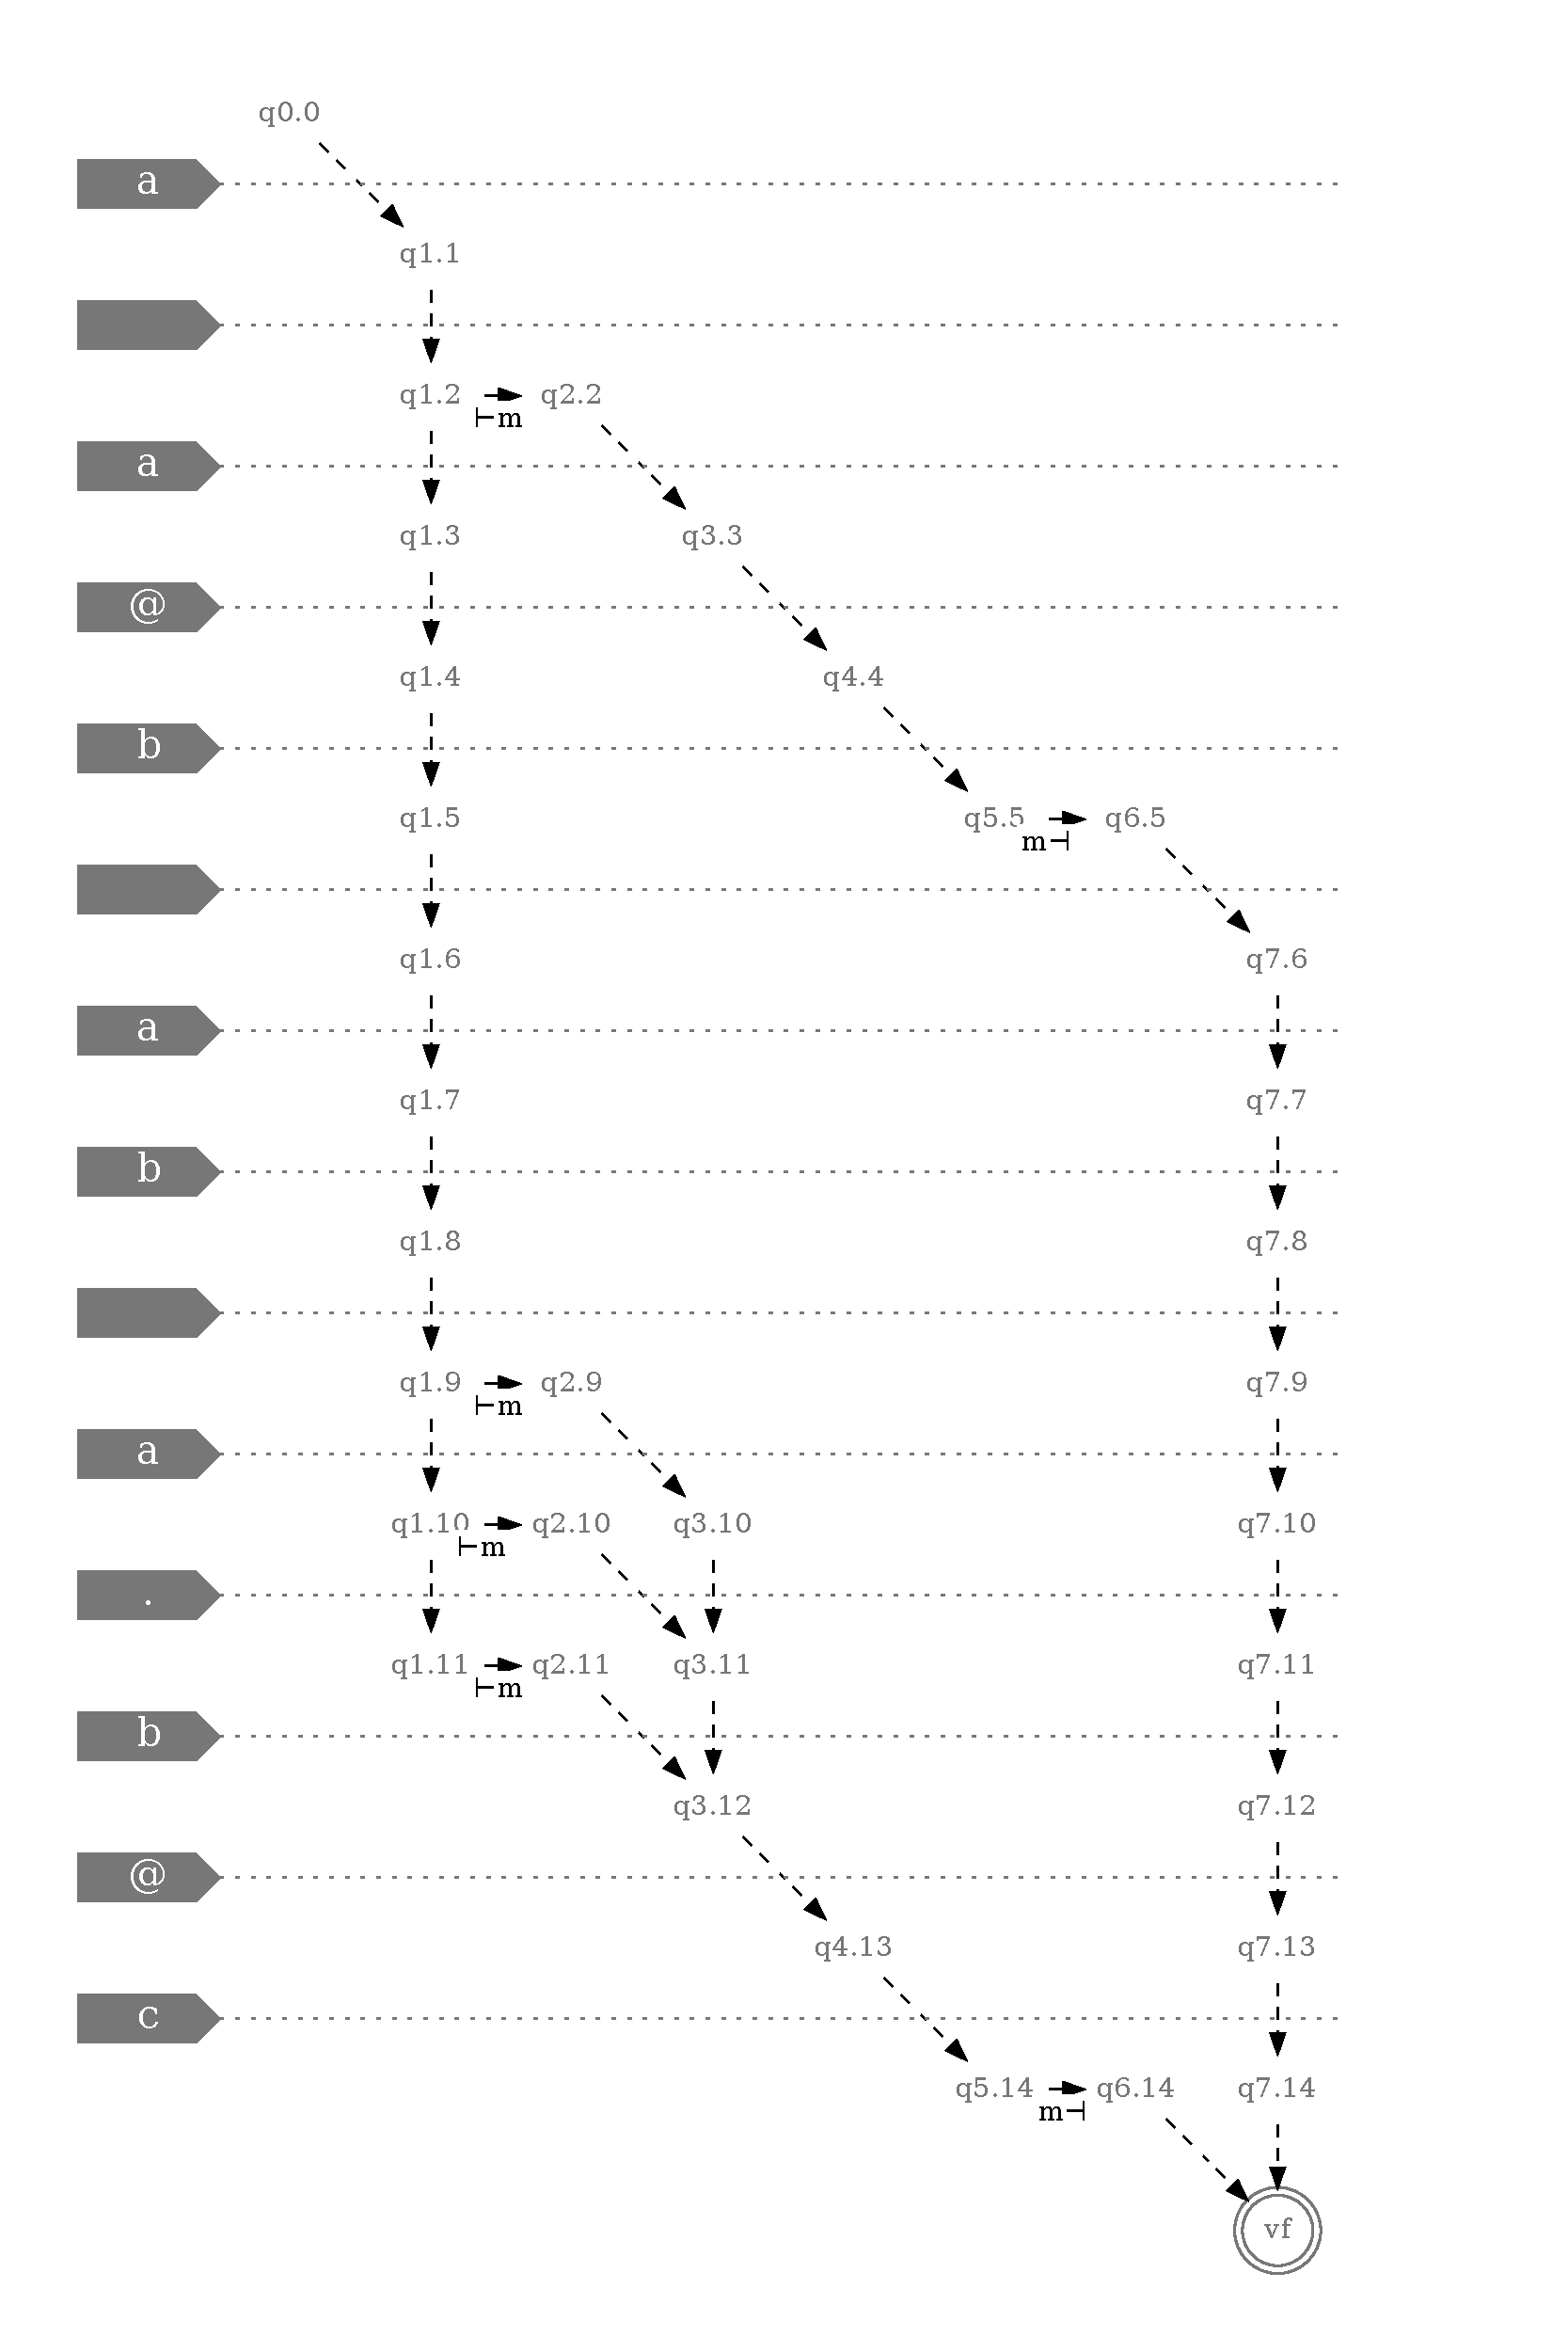
\includegraphics[width=5in]{figures/example_dag}
        \end{figure}

      \subsubsection{Enumeration for mapping DAGs}

        The enumeration over such a DAG is still a non-trivial task to perform.
        The first issue we will face is that we need to make sure that we
        output each mapping at most once, since checking if a mapping is really
        in the output at each step of the enumeration algorithm whould cost
        more that the constant delay we want to achieve.

        To do so, the enumeration is performed by keeping track of a set
        $\Lambda$ of vertices of $G$, included in a single level, together with
        the set \texttt{mapping} of assignations that have been done in the
        paths leading to vertices of $\Lambda$. In other words,
        \texttt{mapping} is the maximal set of pairs $(m, i) \in
        \Gamma_\mathcal{V} \times \mathbb{N}$ such that $(m, i)$ appears
        exactly once in every paths from $v_0$ to a vertex of $\Lambda$.

        Algorithm~\ref{alg:main_enum} describes how this process works. The
        \textproc{Jump} function will be described in next section can be
        considered to be the identity function for the moment without altering
        correctness of the algorithm. The \textproc{NextLevel} function follows
        marker edges inside of a level, enumerating all the pairs
        $(\texttt{locmark}, \Lambda')$ such that \texttt{locmark} is the set of
        the labels read for all paths from a vertex of $\Lambda$ to $\Lambda'$.
        Intuitivelly, \textproc{NextEnum} allows to enumerate all the
        ``choices'' of assignations that can be made inside a level, giving the
        state $\Lambda'$ of the run that such a choice would result to.
        Amarilli \& al.~\cite{ICDT19} introduce a methode to compute
        \textproc{NextLevel} with constant delay by adapting a general approach
        called ``flashlight search''.

        \begin{algorithm}[H]
          \caption{Enumeration from a mapping DAG (\cite{ICDT19} Alg. 1)}%
          \label{alg:main_enum}
          \begin{algorithmic}[1]
            \State{%
              precompute \textproc{JL}, \textproc{rlevel} and \textproc{reach}
            }
            \\
            \Function{enum}{$\Lambda, \texttt{mapping}$}
              \State{$\Lambda' \gets \Call{Jump}{\Lambda}$}
              \If{$\Lambda'$ is the singleton $\{v_f\}$ of the final vertex}
                \State{\textbf{send} \texttt{mapping}}
              \Else{}
                \For{%
                  $(\texttt{locmark}, \Lambda'')$ in
                  \Call{NextLevel}{$\Lambda'$}
                }
                  \State{%
                    \Call{enum}{%
                      $\Lambda'', \texttt{locmark} \cup \texttt{mapping}$
                    }
                  }
                \EndFor{}
              \EndIf{}
            \EndFunction{}
            \\
            \For{mapping \textbf{in} \Call{enum}{$\{v_0\}, \emptyset$}}
              \State{\textbf{output} \texttt{mapping}}
            \EndFor{}
          \end{algorithmic}
        \end{algorithm}

      \subsubsection{The Jump function}

        Intuitively, $\Call{Jump}{\Lambda}$ computes the set of vertices
        $\Lambda'$ that can be reached by following $\epsilon$-edges from
        $\Lambda$ and that all belong first level where a path starting from
        $\Lambda$ can contain a marker transition. This function will allow to
        run Algorithm~\ref{alg:main_enum} with constant delay, by skipng
        efficiently levels where no markers can be added to the mapping.

        The \textproc{Jump} function requires to pre-compute various indexes
        which are defined below.

        \paragraph{jump level}

          \textproc{JL} is defined for all $v \in V$ the minimal level
          containing a vertex $v'$ such that $v'$ is reachable from $v$ and
          $v'$ is either the final vertex or has an outgoing marker edge.

          It can be computed in time $O(D \times W^2)$ by dynamic programming
          and given these relations: $\Call{JL}{v} = level(v)$ if $v = v_f$ or
          if $v$ has an outgoing marker edge, otherwise $\Call{JL}{v} =
          \min\limits_{(v, v') \in E} \Call{JL}{v'}$.

        \paragraph{reachables}

          \textproc{Rlevel} is defined for any level $i$ as follows:
          $\Call{Rlevel}{i} = \{\Call{JL}{v}, level(v) = i\}$. This can be
          computed in time linear in $|G|$ since each vertex belongs to exactly
          one level.

        \paragraph{reachability matrix}

          For any pair of levels $i < j$, $\Call{Reach}{i,j}$ is a boolean
          matrix of size at most $W \times W$ which describe for any pair of
          vertices $(u, v)$ such that $level(u) = i$ and $level(v) = j$ whether
          there is a path for $u$ to $v$ ending with an $\epsilon$-edge.

          We only need to pre-compute $\Call{Reach}{i, j}$ for pairs $(i, j)$
          such that $j \in \Call{Rlevel}{i}$. This can be done in time $O(D
          \times W^{4})$ by using dynamic programming implemented using
          $\Call{Reach}{i, j} = \Call{Reach}{i, i+1} \times \Call{Reach}{i+1,
          j}$.

        \paragraph{} Then, for any set of vertices $\Lambda$ subset of a level
        of $G$, we can compute $\Call{Jump}{\Lambda}$ in time $O(W^2)$ by using
        Algorithm~\ref{alg:jump}.

        \begin{algorithm}[H]
          \caption{The Jump function}%
          \label{alg:jump}
          \begin{algorithmic}[1]
            \Function{Jump}{$\Lambda$}
              \State{$i \gets level(v), \text{ for any } v \in \Lambda$}
              \State{$j \gets \min\limits_{v \in \Lambda} \Call{JL}{v}$}
              \If{$i = j$}
                \State{\Return{$\Lambda$}}
              \Else{}
                \State{$M \gets \Call{Reach}{i, j}$}
                \State{%
                  \Return{$\{u \in V \mid level(u) = j \land (\exists v \in
                  \Lambda, M_{u, v} = \texttt{true})\}$}
                }
              \EndIf{}
            \EndFunction{}
          \end{algorithmic}
        \end{algorithm}

    \subsection{Related work}


  \section{Improvements of the algorithm}

    \subsection{Lowering memory complexity}

      The first issue that raised out of early implementations was that it
      would not be reasonable to explicitly represent the whole DAG as it is
      defined in Section~\ref{sec:mapping_dag}. Indeed, the graph is of size
      $O(|\mathcal{A}| \times |d|)$ and the index of matrices \textproc{reach}
      is of size $O(|d| \times W^3) \simeq O(|d| \times |V|^3)$, early
      implementation showed that this structure did not fit in memory for
      reasonable inputs.

      % \begin{theorem}
      %   Algorithm~\ref{alg:main_enum} can be modified to fit in memory $O(\min(K
      %   \times |\mathcal{V}|, |d|) \times W^3)$ where $K$ is the number of
      %   mappings of $G$.
      % \end{theorem}

      % Even though this modification can still consume as much memory as it did
      % on worst cases, it proved to make a huge difference on practical cases,
      % especially when the output is small or when matches are concentrated in
      % specific parts of the text.

      The following parts will introduce two modifications to the algorithm:
      computing \textproc{JL}, \textproc{Rlevel} and \textproc{Reach} in
      streaming in order to remove $\epsilon$-edges from the graph and removing
      unreachable states while we pre-compute theses structures.

      In practice these modifications proved to be very efficient has they
      allowed the algorithm to run with a memory cost constant in $d$ on most
      cases we studied.

      \subsubsection{Removing $\epsilon$-transitions}

        Notice that $\epsilon$-edges are never used in
        Algorithm~\ref{alg:main_enum} since $\textproc{NextLevel}$ follows
        marker edges only and $\textproc{Jump}$ relies on structures that
        compactify the informations contained in these edges.

        For any $v$ such that $level(v) = i$, $\Call{JL}{v}$,
        $\Call{Rlevel}{i}$ and $\Call{Reach}{i, \cdot}$ are computed by
        recursive formulas that only depend of of the values of \textproc{JL},
        \textproc{Rlevel} and \textproc{Reach} for levels higher than $i$. This
        leads to the following claim:

        \begin{theorem}
          The constructions of \textproc{JL}, \textproc{Rlevel} and
          \textproc{Reach} can be computed with no extra complexity given only
          the input VA $\mathcal{A}$ and the document $d$.
        \end{theorem}

        Algorithm~\ref{alg:build_jl} show how to compute \textproc{JL} at the
        same time as we build $G$ without any $\epsilon$-edge. The algorithm
        can be adapted to compute \textproc{Rlevel} and \textproc{Reach} in a
        similar way.

        \begin{algorithm}[H]
          \caption{Streaming computation of \textproc{JL}}%
          \label{alg:build_jl}
          \begin{algorithmic}[1]
            \State{$V \gets \{v_f\}$}
            \State{$E \gets \emptyset$}
            \State{$\Call{JL}{v_f} \gets |d| + 1$}
            \For{$q$ \textbf{in} $F$}
              \State{$v \gets (q, |d|)$}
              \State{$V \gets V \uplus \{v\}$}
              \If{there is no marker transitions that start from $v$}
                \State{$\Call{JL}{v} \gets |d|$}
              \EndIf{}
            \EndFor{}
            \For{$i = |d|-1$ \textbf{down to} 0}
              \For{$q$ \textbf{in} $Q$}
                \State{$v \gets (q, i)$}
                \State{$V \gets V \uplus \{v\}$}
                \ForAll{$(q, a, q') \in \Delta$}
                  \If{$a$ is a variable marker}
                    \State{$v' \gets (q, i+1)$}
                    \State{$E \gets E \uplus \{(v, (a, i), v')\}$}
                    \State{$\Call{JL}{v} \gets i$}
                  \ElsIf{$a = d_{i+1}$}
                    \State{
                      $\Call{JL}{v} \gets \Call{JL}{v'}$ \textbf{if}
                      $\Call{JL}{v}$ is unassigned \textbf{else}
                      $\min(\Call{JL}{v}, \Call{JL}{v'})$
                    }
                  \EndIf{}
                \EndFor{}
                \State{}
              \EndFor{}
            \EndFor{}
          \end{algorithmic}
        \end{algorithm}

      \subsubsection{Cleaning useless states}

        As vertices that or not accessible or not co-accessible can't be part
        of an accepting path n $G$, they can be removed. This can be done by
        computing two runs over $G$ after it is computed, one starting from the
        initial vertex and one starting from the final vertex. One of the two
        runs can be simulated at the same time as we build $G$, but either the
        accessible or co-accessible states have to be constructed at some
        point.

        Also note that levels of the DAG that do not contain any marker edge
        can also be removed from the DAG since the \textproc{Jump} function
        can't reach them.

        The second optimisation added to the algorithm is then to remove theses
        unreachable nodes as soon as possible, which can be done by keeping
        track of the number of edges starting from a vertex, when a vertex $v'$
        is removed this counter is decremented for every vertex $v$ such that
        there is a marker edge from $v$ to $v'$ or $v'$ is adjacent to $v$ in
        the matrix $\Call{Reach}{level(v), level(v')}$.

        Note that sadly this modification can still be has bad as the
        unmodified algorithm, for example the graph obtained with the regex
        \texttt{a*x\{a\{1000\}\}a*} over the document $d = aa \ldots aab$ will
        only contain accessible vertices, except for vertices of the last
        level.  Thus the compression operation will not be able to perform
        until the last letter of $d$ is read.

  \section{Performance of the algorithm}

    \subsection{Implementation}

      A first draft of the implementation of the algorithm was implemented
      using Python~3~\cite{implPython}, and a later efficient implementation
      was rewritten using Rust~\cite{implRust}.

      These implementations are built by a succession of supersteps:
      \begin{enumerate}
        \item a parser for the syntax of regex formulas, that convert an input
          regular expression into an abstract syntax tree (AST);
        \item an algorithm to compile this AST into an automaton; here
          Glushkov algorithm is used, modified as explained in
          Section~\ref{sec:regex_formula};
        \item the pre-computation of our enumeration algorithm, that compiles
          the matches of the automaton over a document into a compact
          structure;
        \item the enumeration over this structure.
      \end{enumerate}

      The main unnecessary overhead of the implementation as it stands is that
      it saves all vertex-related informations in an hash table data structure
      in order to efficiently deal with the sparsity of the graph, and with the
      fact that we must be able to delete vertices efficiently. Some of theses
      structures may be replaceable with a low-level array, which would
      decrease the constant cost of accessing these hash tables and the
      corresponding memory usage.

      The cleaning of useless states is implemented by running a pass after
      building each level. After building level $i$ it would remove useless
      states in the last $2^k$ levels for the highest $k$ such that $2^k$
      divides $i$. This adds a logarithmic $O(\log |d|)$ factor but allows to
      update \textproc{Reach} matrices less often, which is in practice rather
      slow since it requires to perform a memory allocation.

    \subsection{Limitations of existing tools}

      Except for the naive algorithms and the work of Florenzano et
      al.~\cite{florenzano2018constant} \pierre{These should really be
      discussed as a separate subsection}, it is difficult to fairly compare to
      already existing tools. First, we will limit our tests to
      Problem~\ref{pb:weak} in order to be able to compare the speed of our
      algorithm with existing tools.

      Some of these tools \pierre{Which tools? You really need to discuss
      existing tools in detail} allow to output a list of overlapping matches,
      however this will at most output one match for each starting position in
      the output document. Regular expressions actually have a greedy semantic
      for closures in the context of these tools, it will as a default match
      the largest possible string for each closure and can be turned to a lazy
      semantic where it only matches the smallest possible string. For example
      over the text \texttt{abcde} by using GNU grep \pierre{How do you use
      grep to return multiple matches? Don't you want to refer to another
      implementation?}:
        \begin{itemize}
          \item the regexp \texttt{...*} will output \texttt{abcde},
            \texttt{bcde}, \texttt{cde}, \texttt{de};
          \item the regexp \texttt{...*?} (where \texttt{*?} is the lazy
            version of \texttt{*}) will output \texttt{ab}, \texttt{bc},
            \texttt{cd} and \texttt{de}.
        \end{itemize}
      However, the output to the enumeration problem should contain all
      substrings of size at least 2, thus these two kinds of greedy semantics
      don't need to be treated separately. \pierre{This is not the main
      message I get: I get more that these semantics are not appropriate}

      We will still compare our results with these tools but we need to
      keep in mind that their output will be a subset of the output of our
      algorithm.

    \subsection{Results}

      We compared performances of several tools: our Rust implementation
      (\texttt{dag\_rs}) and Python implementation (\texttt{dag\_py}), the
      implementation of the algorithm of Florenzano et al.
      \cite{florenzano2018constant} (\texttt{SpannerConst}) \pierre{Say where
      you found it}, naive algorithms running in time $O(\mathcal{A} \times
      |d|^2)$ and $O(|d|^3)$ \pierre{Again, they need to be described} and
      finally, \texttt{grep} and \texttt{ripgrep} \pierre{Again, they need to
      be described} will serve as our reference of pre-existing tools.

      The results of Figure~\ref{fig:bench} are quite representative of all the
      results we got. The enumeration phase is very quick for our
      implementation, the delay has never been measured to be greater than $50
      \mu s$ (which gives a bandwidth greater than $2 \times 10^4$ matches/s).
      As expected \texttt{grep} and \texttt{ripgrep} output less overlapping
      matches than \texttt{SpannerConst} and our tool do.

      The preprocessing phase is always much slower than the enumeration phase
      and is the limiting part of the algorithm. Naive algorithms seem more
      relevant than this tool when it comes to getting quickly a small subset
      of the matches, but can't compete with a linear time algorithm on
      outputting all the matches.

      We noticed that \texttt{SpannerConst} is faster than our approach on most
      cases, usually by a factor greater than 10. However the approach of the
      algorithm relies on determinized automata on examples where an input
      regex is very hard to determinize, the exponential cost of determinizing
      this regex exceeds by far the time spent
      processing~(Figure~\ref{fig:hard_determinisation}).


      \begin{figure}%
        \caption{
          Enumeration speed for our implementation (\texttt{dag\_rs}),
          $R_1$~(\ref{sec:regex_glossary}), input document: 10MB of DNA }
        \center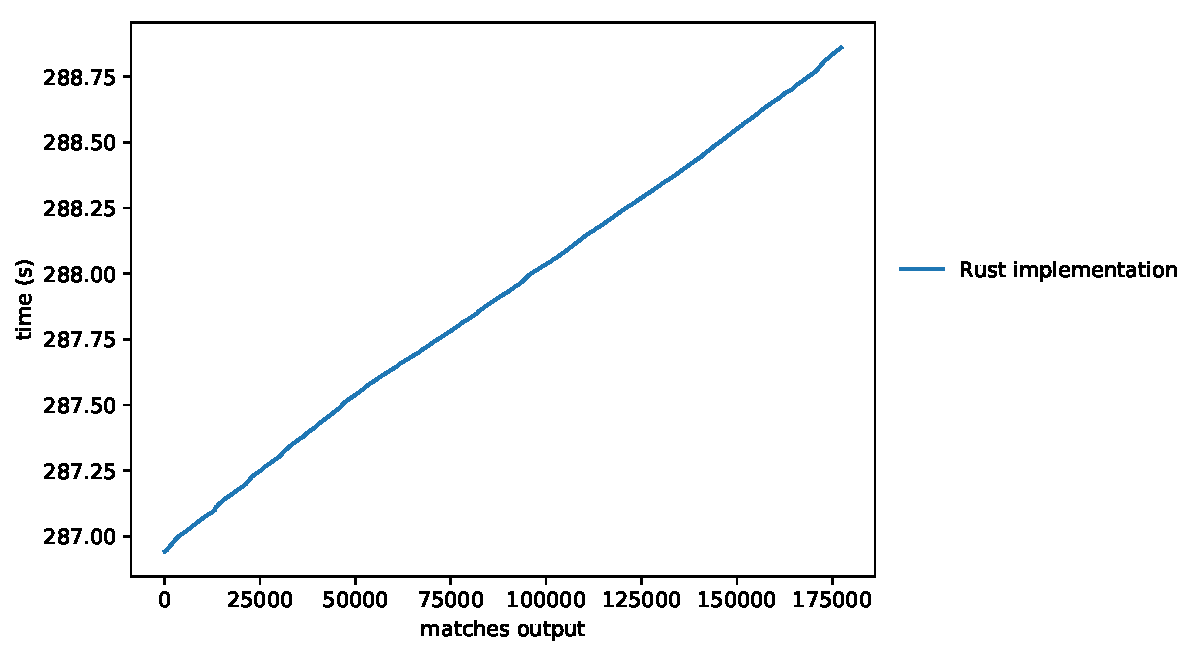
\includegraphics[width=5in]{figures/bench_enum_only}

        \pierre{In the axis legend, ``outputed yet'' should be
        ``output''}
      \end{figure}

      \begin{figure}%
        \caption{
          Enumeration speed of the different algorithms, input regex:
          $R_1$~(\ref{sec:regex_glossary}), input document: 10MB of DNA
        }
        \label{fig:bench} \pierre{Same label as previous figure???}
        \center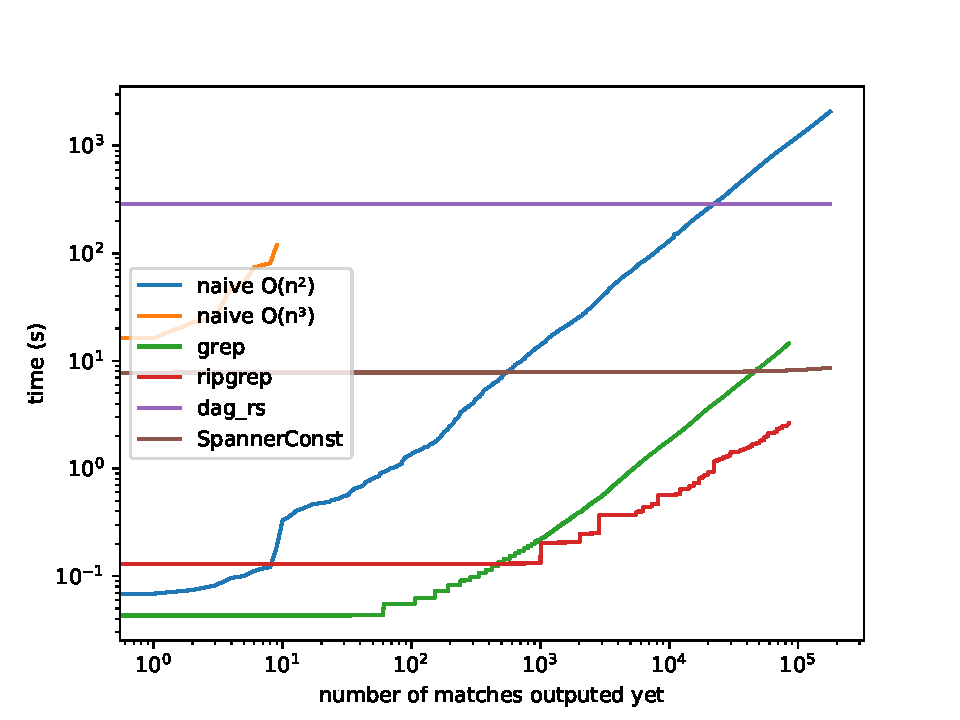
\includegraphics[width=5in]{figures/bench}
        \pierre{In the axis legend, ``outputed yet'' should be
        ``output''}
        \pierre{Move the key somewhere it does not overlap with the
        graphs...}
      \end{figure}

      % \begin{figure}%
      %   \label{fig:bench}
      %   \caption{}
      %   \center\includegraphics[width=5in]{figures/hard_determinisation}
      % \end{figure}


  \section{Conclusion}

    The work of this internship enriched the algorithm described
    in~\cite{ICDT19} to make it usable in practice.

    Even though the chosen approach of not determinizing the input automaton
    allows to avoid an exponential factor in the size of this automaton, it
    doesn't seem to pay off compared to a determinized approach such as the
    algorithm described by Florenzano et al.~\cite{florenzano2018constant}.

  \pagebreak
  \bibliography{bibliography}
  \bibliographystyle{ieeetr}


  \pagebreak
  \section*{Appendices}

    \todo[inline]{Maybe Glushkov here?}

    \subsection{Naive algorithm for the weak problem}

      The algorithm bellow can be implemented in time $O(|d|^2 \times |Q|)$ for
      a NFA by using an efficient index to access $\Delta$. It can be
      implemented in time $O(|d|^2)$ for a DFA\@: since at any step of the
      algorithm $|S| = 1$, lines 5 and 7 can be implemented in constant time.

      \begin{algorithm}[H]%
        \label{alg:naive}
        \begin{algorithmic}[1]
          \State{$\texttt{output} \gets \emptyset$}
          \For{$i = 0$ to $|d|$}
            \State{$S \gets \{q_\text{init}\}$}
            \For{$j = i$ to $|d|$}
              \If{$S \cap F \neq \emptyset$}
                \State{%
                  $\texttt{output} \gets \texttt{output} \uplus \{\Span{i,
                  j}\}$
                }
              \EndIf{}
              \State{%
                $S \gets \{q' \in Q, \exists q \in S, (q, d_j, q') \in \Delta
                \}$
              }
            \EndFor{}
          \EndFor{}
        \end{algorithmic}
        \caption{%
          A naive quadratic algorithm for Problem~\ref{pb:weak} with inputs
          $\mathcal{A} = (Q, q_\text{init}, \Delta, F)$ and $d \in \Sigma^*$
        }
      \end{algorithm}

    \subsection{Regex glossary}%
      \label{sec:regex_glossary}

\end{document}
